\documentclass[a4paper,12pt]{article}

% Packages nécessaires
\usepackage[utf8]{inputenc}
\usepackage[T1]{fontenc}
\usepackage[french]{babel}
\usepackage{graphicx} % Pour inclure des images
\usepackage{caption} % Pour personnaliser les légendes
\usepackage{array} % Pour les tableaux
\usepackage{mathpazo} %police pas mal
%\usepackage{lmodern} % Police Latin Modern
\usepackage{amsmath} % Pour les formules mathématiques
\usepackage{geometry} % Pour ajuster les marges
\usepackage{fancyhdr} % Pour personnaliser les en-têtes et pieds de page
\usepackage{tikz} % Pour les images en arrière-plan
\usepackage{lipsum} % Pour générer du texte d'exemple
\geometry{top=4cm, bottom=2.5cm, left=2.5cm, right=2.5cm, headheight=2cm, headsep=1cm}

% Début du document
\begin{document}

% Page de titre
\begin{titlepage}
    \begin{minipage}[t]{0.4\textwidth}
        
\includegraphics[width=\textwidth]{media/logo-enit-2454399073.png} \\[1cm] % Logo de l'établissement
    \end{minipage}
    \centering
    \vspace*{2cm}
    \begin{tikzpicture}[remember picture, overlay]
        \node[opacity=0.2, anchor=south] at (current page.south) {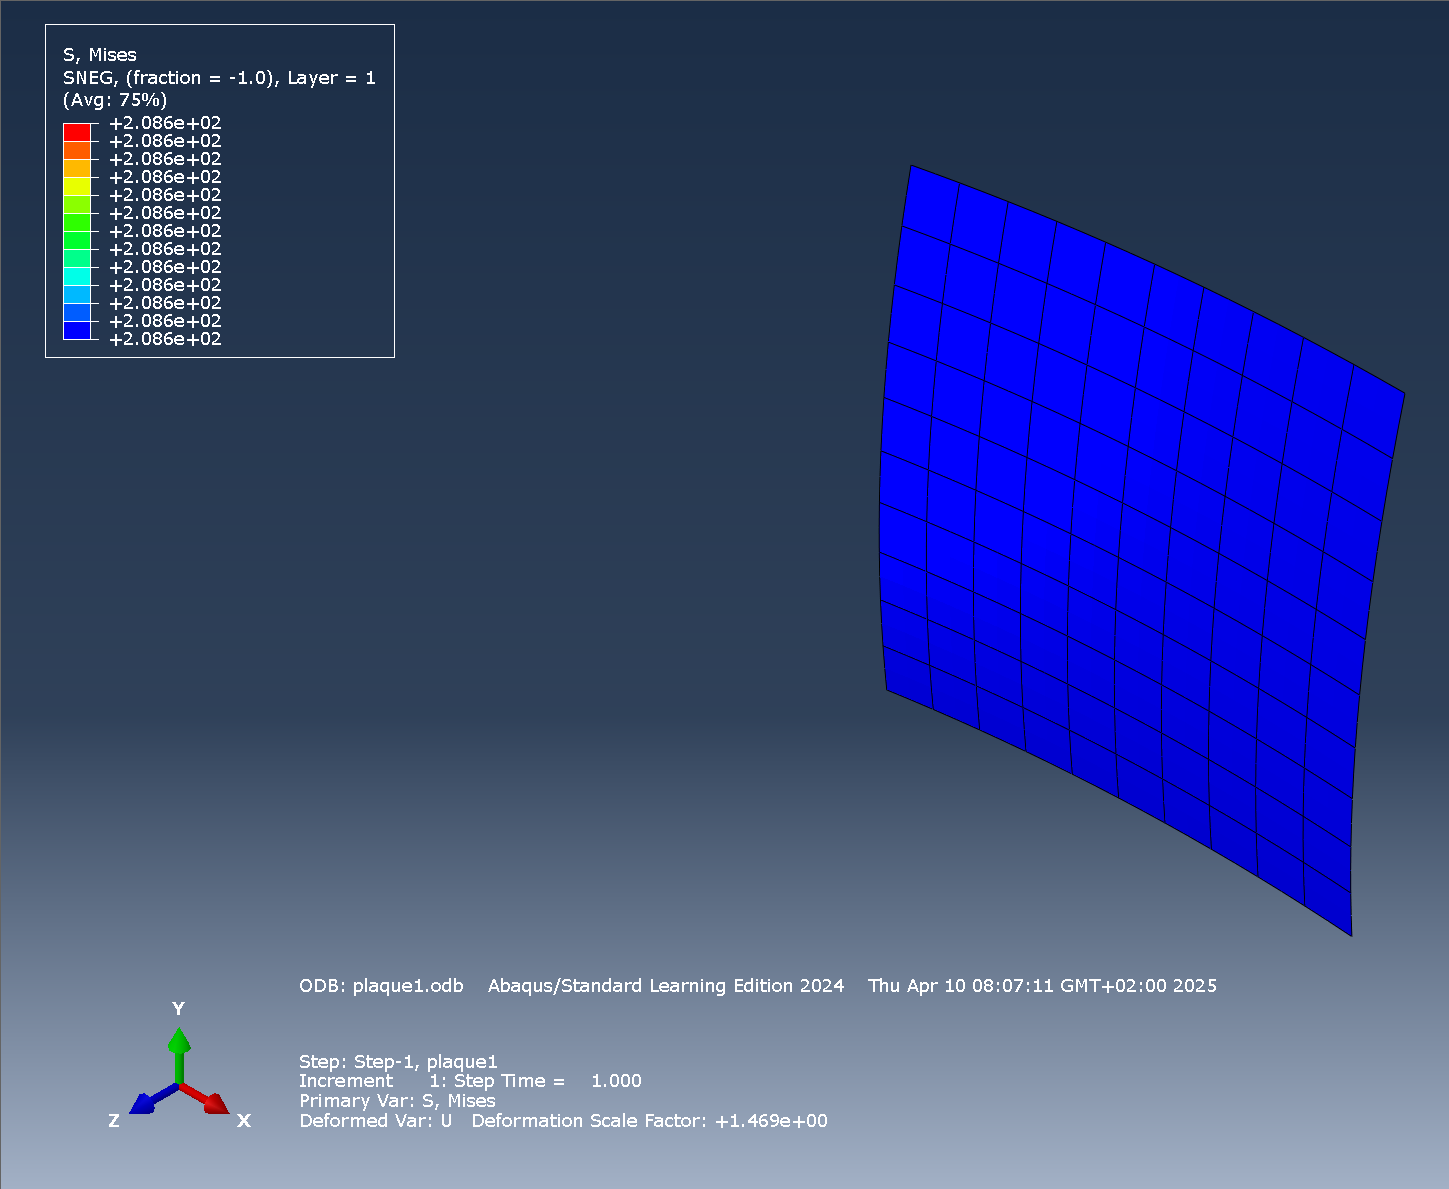
\includegraphics[width=1\paperwidth]{media/page de garde.png}}; % Image d'arrière-plan
    \end{tikzpicture}
    
    {\scshape \Large Rapport de TP Universitaire} \\[0.5cm] % Type de document
    {\Huge \textbf{Titre du TP}} \\[1.5cm] % Titre du TP
    {\large \textbf{Killian RENOU \\ William GUILBERT}} \\[0.5cm] % Noms des auteurs
    {\large \textbf{Date : 20/10/2023}} \\[0.5cm] % Date
    {\large \textbf{ENIT - École Nationale d'Ingénieurs de Tarbes}} \\[0.5cm] % Établissement
    \vfill
    {\large \textbf{Encadrant : Nom de l'encadrant}} % Nom de l'encadrant
\end{titlepage}


% Configuration des en-têtes et pieds de page
\pagestyle{fancy}
\fancyhf{} % Efface les en-têtes et pieds de page par défaut
\fancyhead[L]{
\includegraphics[width=3cm]{media/logo-enit-2454399073.png}} % Logo à gauche
\fancyhead[C]{\textbf{Rapport de TP Universitaire}} % Titre au centre
\fancyhead[R]{\textbf{ Killian RENOU  \\ William GUILBERT }} % Noms à droite, l'un sous l'autre
\fancyfoot[R]{\thepage} % Numéro de page centré en pied de page
\renewcommand{\headrulewidth}{0.4pt} % Ligne noire sous l'en-tête

% Table des matières
\tableofcontents
\newpage

% Introduction
\section{Introduction}
Dans cette section, introduisez le sujet du TP, les objectifs et le contexte.

% Matériel et méthodes
\section{Matériel et Méthodes}
Décrivez les équipements utilisés, les protocoles suivis et les étapes principales.

% Résultats
\section{Résultats}
\subsection{Exemple d'image avec légende}
\begin{figure}[h!]
	\centering
	
\includegraphics[width=0.7\textwidth]{media/logo-enit-2454399073.png} % Remplacez par le chemin de votre image
	\caption{Exemple de légende pour une image.}
	\label{fig:exemple_image}
\end{figure}

\subsection{Exemple de tableau}
\begin{table}[h!]
	\centering
	\begin{tabular}{|c|c|c|}
		\hline
		\textbf{Paramètre} & \textbf{Valeur} & \textbf{Unité} \\
		\hline
		Exemple 1          & 10              & m/s            \\
		Exemple 2          & 20              & m/s            \\
		Exemple 3          & 30              & m/s            \\
		\hline
	\end{tabular}
	\caption{Exemple de tableau avec des données.}
	\label{tab:exemple_tableau}
\end{table}

% Discussion
\section{Discussion}
Analysez les résultats obtenus, discutez des erreurs possibles et proposez des améliorations.

% Conclusion
\section{Conclusion}
Résumé des résultats principaux et conclusion générale.

% test de corp de texte
\section{Test de corps de texte}
\lipsum[1-3] % Génère trois paragraphes de texte d'exemple

% Bibliographie
\section*{Bibliographie}
\begin{itemize}
	\item Référence 1
	\item Référence 2
\end{itemize}

\end{document}